In this section we will focus on the benchmarks
and the more tangible results of the project.
To start, lets take a look at \autoref{fig:pillar-plot}.

\begin{figure}[hbtp]
	\centering
	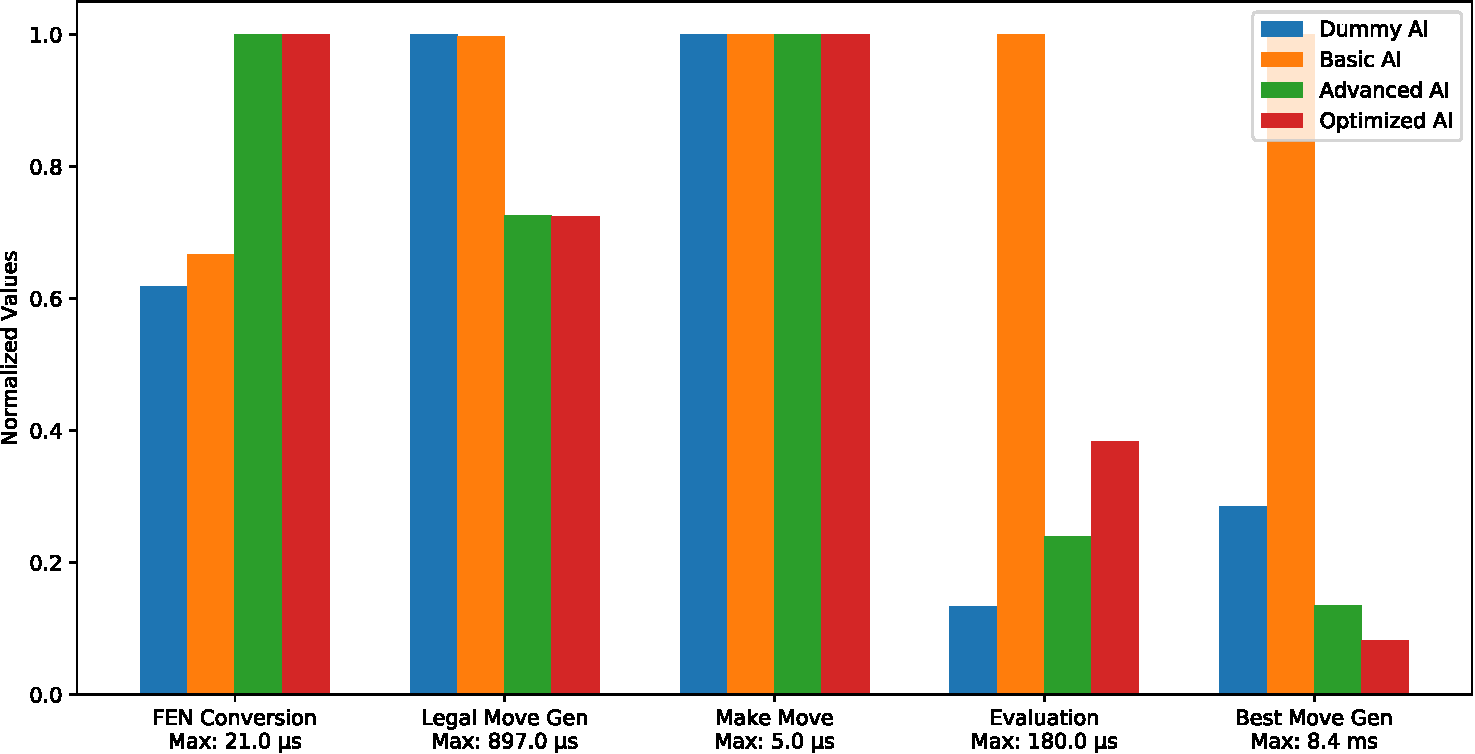
\includegraphics[width=.9\linewidth, page=1]{reference/pics/plot.pdf}
	\caption{Benchmarks of the different categories across the AI versions.}
	\label{fig:pillar-plot}
\end{figure}

We can see five categories, of which the first three
are determined by the chess backend and the later two
by the AI.
Important to note in the backend benchmarks is the legal move
generation. This is the main bottleneck of the backend
and a increasing the performance there has quite
the effect on the overall performance of the AI.
The decrease in time stems from the refactor of using
lists of integers and reducing boilerplate\footnote{
The Fen conversion is only used for debugging
purposes, the fact that it increased is not noticeable
in an optimized AI that doesn't debug anything.}.
The most important category however is the last one,
the \textit{Best Move Generation}. As the name suggests,
this indicates how fast the AI calculated the best move,
here at a depth of one.
The optimized AI has the best overall time,
even though it's slower in the evaluation compared to
the previous version. This illustrates very nicely
that the end result of an AI, it's strength and speed,
is determined by multiple factors. In this case
the amount of nodes searched was drastically decreased
by the AI features implemented which led to this
overall improvement. This leads us to \autoref{fig:depth-plot}, which shows
the time and number of nodes searched in respect to the
depths.

There we can see numbers of nodes searched (bottom plot) is significantly
lower for the optimized AI compared to the advanced AI\footnote{
The reason the dummy and basic AI seem to have less nodes searched
is because there was a bug in the early implementations of the AI.
This bug had to do with the move ordering and was fixed in milestone three.
For that reason the dummy and basic AI's benchmarks in regard to depth
should be taken with a grain of salt.
}. We can also see that the overall time is smaller for the optimized AI,
regardless of depth.

\pagebreak

This is actually not necessarily the case,
for instance if we would have made poor decisions for the MCTS
with regard to exploration/exploitation and this could have actually been
slower for higher depths. This is where regular benchmarks, or atomic
benchmarks are very useful, you change one little nod and see how the
system responds. Research also helped to fine tune.

\begin{figure}[hbtp]
	\centering
	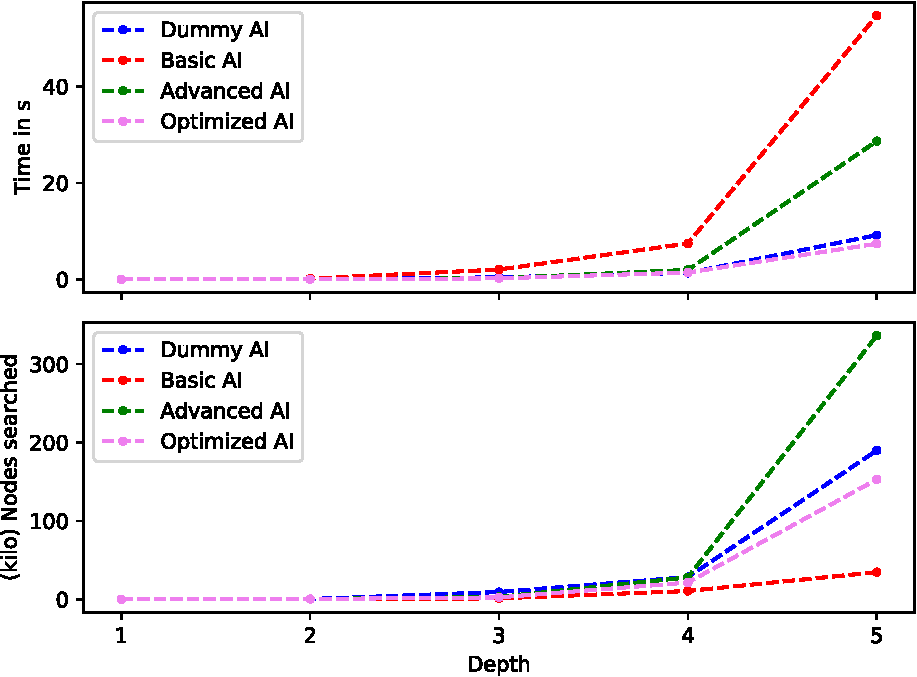
\includegraphics[width=.8\linewidth, page=1]{reference/pics/plot-depths.pdf}
	\captionsetup{justification=centering}
	\caption{Benchmarks of different AI versions in respect to search depth.\\Note that the number of nodes searched is in thousands (kilo).}
	\label{fig:depth-plot}
\end{figure}

\pagebreak
